\chapter{Powiązania uczenia maszynowego i neuronauki}

\section{Hipotezy w kierunku integracji głębokiego uczenia oraz neuronauki}

Jak zostało opisane w \hyperref[sec:differences]{sekcji \ref*{sec:differences}}, po początkowej obustronnej kooperacji między uczeniem maszynowym oraz neuronauką zaczęły pojawiać się rozbieżności.
Uczenie głębokie skupiło się na ścisłej optymalizacji funkcji kosztu przy stosunkowo jednolitej architekturze.
W neuronauce z kolei to zmienna i złożona architektura, dynamika i systemy mózgowe były w centrum zainteresowania i rozwoju dziedziny.

Jednak nowe technologie w zakresie uczenia maszynowego dają możliwość i nadzieję na ponowne zestawienie ze sobą tych dziedzin.
Zaczęto używać funkcji kosztu znacznie bardziej złożonych i zróżnicowanych warstwami i względem czasu \cite{gulccehre2016knowledge, saxe2013exact};
Pojawiły się architektury ustrukturyzowane, w tym wykorzystujące dedykowane systemy pamięci krótko- i długo-terminowych czy uwagowych (LSTM \cite{chung2014empirical}, adresowalne lokacją czy zawartością \cite{graves2014neural} oraz inne).

Takie idee dotychczas pojawiały się ekskluzywnie w uczeniu maszynowym.
W niedawnej pracy badawczej zostały zaproponowane trzy hipotezy odnoszące się do działania mózgu \cite{marblestone2016toward}, które -- jeśli okazałyby się prawdziwe -- mogłyby prowadzić do ponownej integracji dziedzin uczenia maszynowego i neuronauki.

\subsection{Mózg optymalizuje funkcje kosztu}

Jeśli ma się okazać, że rzeczywiście uczenie maszynowe i neuronauka mogą być na drodze ponownej integracji, to przede wszystkim muszą mieć zgodne podstawy strukturalne.
W uczeniu głębokim taką niezaprzeczalną podstawą jest funkcja kosztu i proces jej optymalizacji.
Pierwsza, zasadnicza hipoteza wspomnianej pracy \cite{marblestone2016toward} mówi, że mózg również optymalizuje funkcję kosztu.

Optymalizacja sama w sobie nie jest niczym nowym w ujęciu działania mózgu.
Chociażby wykorzystanie energii przy funkcjach motorycznych jest bliskie optymalnemu \cite{taylor2011does}.
Nie odnosi się to jednak tylko do funkcji wysokiej abstrakcji, rezultaty innych badań potwierdzają, że podstawowe elementy budowy mózgu, które pojawiły się w procesie ewolucji służą optymalizacji wydajności transmisji sygnału \cite{paprocki2020optimizing}.

Mimo to ta sformułowana hipoteza może budzić wątpliwości.
Czym bowiem tak na prawdę miałaby być ta funkcja kosztu i w jaki sposób ta optymalizacja miałaby przebiegać?
W uczeniu maszynowym rolę optymalizacji najczęściej przyjmuje algorytm propagacji wstecznej błędu.
Takie podejście w dosłownym jego znaczeniu jest oczywiście niemożliwe do realizacji w mózgu, wymaga bowiem reprezentacji liczbowych w celu kalkulacji pochodnych tworzących gradient funkcji.
Jednak ta hipoteza opiera się na ogólniejszym pojęciu optymalizacji z dwiema tezami:

\begin{itemize}
	\item Mózg posiada mechanizmy odpowiadające za przydzielanie wyniku (\emph{credit assignment}), która pozwala mu odpowiednio poprawiać właściwości;
	\item Mózg posiada mechanizmy pozwalające mu na dobór odpowiedniej funkcji kosztu lub jej modyfikację.
\end{itemize}

Te dwie tezy stojące za hipotezą, że móżg optymalizuje funkcje kosztu są możliwe do podparcia przez kilka możliwych, różnych od siebie solucji.

Jedna z nich odchodzi od idei mechanizmów optymalizacyjnych opierających się na gradiencie (\emph{gradient descent}) czy przydzielaniu wyników sieci.
Zamiast tego skupia się na możliwości, że wspomniane tezy są realizowane na basie lokalnej samo-organizacji.

\subsection{Funkcje kosztu mózgu są zróżnicowane względem obszaru i w czasie}

\subsection{Mózg posiada wyspecjalizowane systemy dla kluczowych zadań}

\section{Wpływ powiązań architektonicznych na uczenie maszynowe i neuronaukę}

\subsection{W kierunku rozwoju uczenia głębokiego i maszynowego}

\subsection{W kierunku rozwoju neuronauki}

% \begin{figure}[ht]
% 	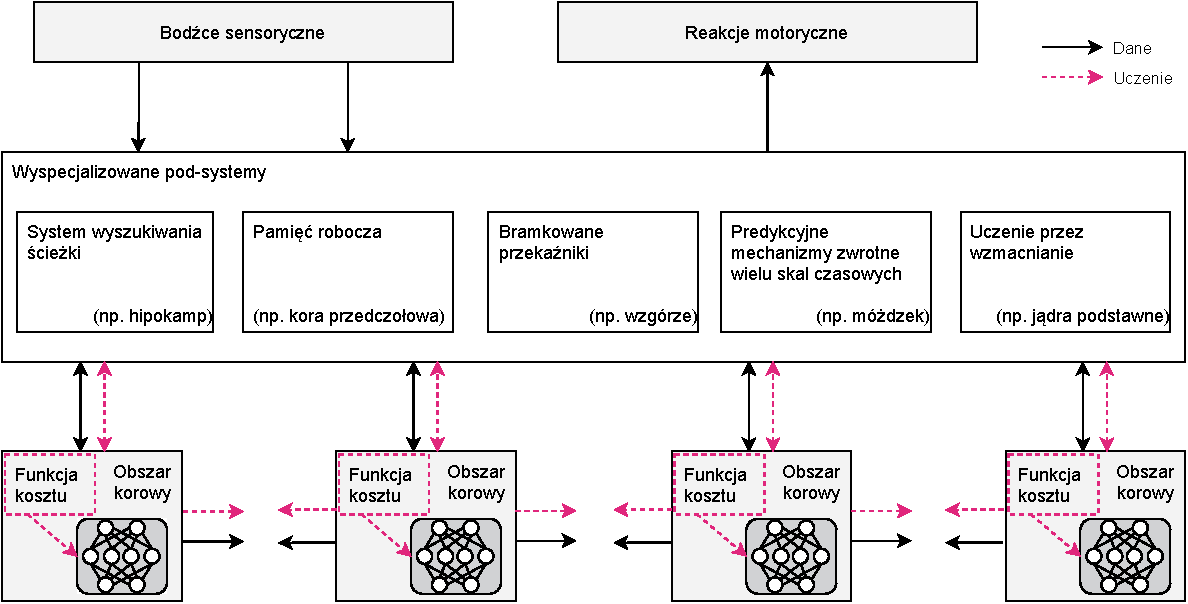
\includegraphics[width=\textwidth]{BrainLikeNeuralNetworkArchitecture.pdf}
% 	\caption{Prawdopodobna struktura systemowa przetwarzania danych i uczenia sieci funkcjonalnych mózgu \cite{marblestone2016toward}}
% 	\label{fig:experiment}
% \end{figure}
